% Owner: Member C (Eesha Irfan).
% Local font encoding restores the template's Times regular/bold faces under XeTeX.
\begingroup
\renewcommand{\encodingdefault}{T1}
\fontencoding{T1}\selectfont
\chapter{High-Level and Low-Level Design}

System design translates requirements into component responsibilities, interfaces and information relationships. The following sections present architectural decisions, subsystem interactions, structural models and behavioural flows, showing how data and control move between the application and its supporting services.

\section{System Overview}

The physician workspace presents patient history, editable consultation notes, specialist findings and clinical drafts in a connected encounter context. Application services validate account access and check that the patient belongs to the requesting physician before retrieving or processing related records. Behind these services, eight agents divide patient-memory retrieval, case preparation, imaging, laboratory processing, medication review, evidence retrieval, clinical reasoning and critic review. Their outputs retain source identifiers and processing states so incomplete analysis does not become an apparent finding. PostgreSQL stores account, encounter, revision and decision relationships, while pgvector supports semantic retrieval over authorised sources. Generated content remains a draft until the physician accepts its reviewed revision. Modification creates a pending revision, and rejection retains the action without creating an accepted decision. Audit records connect each review action to its actor, time and encounter. Research outputs remain separate from accepted decisions even when an evaluation uses the same encounter context.

\section{Design Considerations}

Component boundaries must accommodate different clinical representations without losing patient ownership or source context. Consultation audio needs an incremental capture path, imaging requires model-compatible preparation, and laboratory and medication information require interpretable structured inputs. External model or knowledge services can fail independently, so their status and errors must remain visible to the application. Historical retrieval must distinguish source observations from accepted decisions and prevent another physician's records from entering the case. Draft preparation needs revision-specific evidence and critic findings, while approval requires the accepted content to match the saved revision. These concerns guide the division between interface, application gateway, orchestration, analytical services and persistence. Design choices need to support controlled research comparisons without treating components as automatically beneficial. Numerical latency limits, hardware capacity, model selection and resource coverage depend on the eventual environment. Consequently, the design specifies responsibilities and failure boundaries while leaving configuration-dependent values to documented selection and measurement.

\subsection{Assumptions and Dependencies}

The direct clinical user is a physician who can interpret patient information and assess generated recommendations. The interface assumes a supported web browser, permission to capture consultation audio when recording is used, and connectivity to whichever processing services are selected. Patient cases are de-identified or synthetic, and each patient has one responsible physician for access control. Imaging analysis depends on a validated model whose task and input requirements match the chosen clinical domain. Transcription, embeddings, evidence retrieval and medication review depend on suitable resources and permitted use. PostgreSQL transactions and pgvector provide the relational and semantic storage capabilities. LangGraph and Google ADK are identified orchestration technologies, but their responsibility split requires an implementation decision rather than an assumed combined engine. These dependencies must be recorded with versions, configuration and limitations before comparative runs. A missing dependency should produce an identifiable unavailable state, not an invented finding or implied successful analysis.

\subsection{General Constraints}

Zeest provides clinical assistance rather than autonomous treatment or prescribing. Generated diagnoses and treatment plans remain reviewable drafts, and no agent can create an accepted decision through inference alone. Account and ownership checks govern every clinical read and processing request, including related inputs, drafts and audit actions. Development uses permitted de-identified or synthetic cases; this restriction does not establish regulatory approval or suitability for real clinical deployment. Existing imaging models define their own tasks, and unsupported inputs must be rejected or shown as unavailable. Computational requirements depend on the selected services and case collection, so the architecture cannot claim guaranteed throughput or query latency. Saved input and draft revisions preserve provenance across corrections and review. The same restrictions apply to evaluation configurations: cases, source permissions and reference procedures must be documented. Restrictions apply to all analytical paths, including failed requests and partially completed cases that remain available for physician inspection.

\subsection{Goals and Guidelines}

The design prioritises understandable context, traceable sources, physician control and maintainable component interfaces. Patient and encounter identifiers remain available throughout the workflow so that an operation cannot silently act on a different case. Clinical inputs, specialist findings, retrieved passages, critic findings and generated drafts have representations and display states. Approval controls identify the reviewed revision, while modification and rejection preserve their separate consequences. Analytical components exchange typed information with source references and error status rather than relying on unstructured handoffs alone. Compatible models can be replaced through adapters after their inputs and outputs are checked against these contracts. Failure handling should expose unavailable or incomplete stages without manufacturing clinical conclusions. Evidence retrieval and critic review support inspection but do not guarantee correctness or eliminate hallucinations. Research configurations preserve the same case definitions and assessment process across comparisons. Their value depends on verified behaviour rather than the number of connected components.

\subsection{ Development Methods}

Development follows the requirements, use-case definitions and logical data relationships established in Chapter~4. The initial work defines component contracts, account ownership checks and input and draft revisions before connecting model services. Small integration stages then establish patient navigation, consultation notes, specialist processing, evidence retrieval and the review boundary. Structural and behavioural diagrams describe responsibilities, messages and permitted state transitions, while test cases examine normal operations and rejected requests. Changes to an analytical component must preserve patient, encounter and source associations and expose any new input restrictions. Methodological comparisons use configurations so architecture changes can be distinguished from changes to cases or assessment conditions. The process keeps resource selection explicit: candidate datasets, knowledge sources and models require permission and domain checks before use. Implementation claims must follow working integration, and performance claims must follow measurements. The saved configuration identifies which resources and case restrictions governed each integration or evaluation run.

\section{System Architecture}

Figure~\ref{fig:esha:d07} separates the physician interface, application gateway, agent orchestration and supporting services. Next.js provides the web interface, and FastAPI provides the Python application boundary.~\cite{zeestC:nextjs,zeestC:fastapi} The gateway handles authentication, patient ownership, validated requests and revision-aware decision operations before dispatching analytical work. LangGraph and Google ADK inform the orchestration design; their exact division remains an implementation choice.~\cite{zeestB:langgraph,zeestB:googleadk} Model adapters connect consultation transcription, existing imaging classifiers and Gemini-based reasoning without exposing internal services directly to the browser.~\cite{zeestC:pytorch,zeestC:gemini} PostgreSQL preserves relational records, and pgvector supports semantic retrieval.~\cite{zeestC:pgvector} Streaming communication serves consultation capture, while transactional requests serve saved case operations and physician decisions. Failures return status rather than implied findings. Draft preparation and accepted-decision recording follow different paths, so analytical assistance cannot bypass explicit approval. The architecture describes intended service responsibilities; deployment capacity, latency and runtime configuration require implementation and measurement.  Analytical services return source-aware outputs without acquiring authority to accept a clinical decision.

\begin{figure}[!htbp]
\centering
\includegraphics[width=\textwidth,height=0.80\textheight,keepaspectratio]{Figures/esha_D07_system_architecture.pdf}
\caption{Zeest interface, gateway, agents, analytical services and hybrid memory.}
\label{fig:esha:d07}
\end{figure}

\subsection{Subsystem Architecture}

Figure~\ref{fig:esha:d08} groups the eight agents by their contributions to case preparation, specialised analysis and draft review. The Patient Memory Agent retrieves source-aware history, and the Clinical Case Agent combines it with current saved inputs. Imaging, Laboratory and Medication Safety agents return findings or explicit failure states for supported inputs. The Evidence and RAG Agent supplies cited passages, the Clinical Reasoning Agent creates a diagnosis and treatment draft, and the Safety and Critic Agent identifies concerns before presentation. Table~\ref{tab:esha:contracts} defines these handoffs. Figure~\ref{fig:esha:d10} follows consultation capture through note correction, analysis and physician presentation; Figure~\ref{fig:esha:d12} follows modification, approval and rejection through persistence. Independent analyses may run concurrently where their dependencies permit, but downstream reasoning must identify incomplete stages. Authorised input revisions and approved decisions can supply semantic memory; pending drafts cannot enter it as accepted clinical facts. These contracts preserve the distinction between preparation, recommendations and recorded decisions. Their outputs require verification.

\begin{figure}[!htbp]
\centering
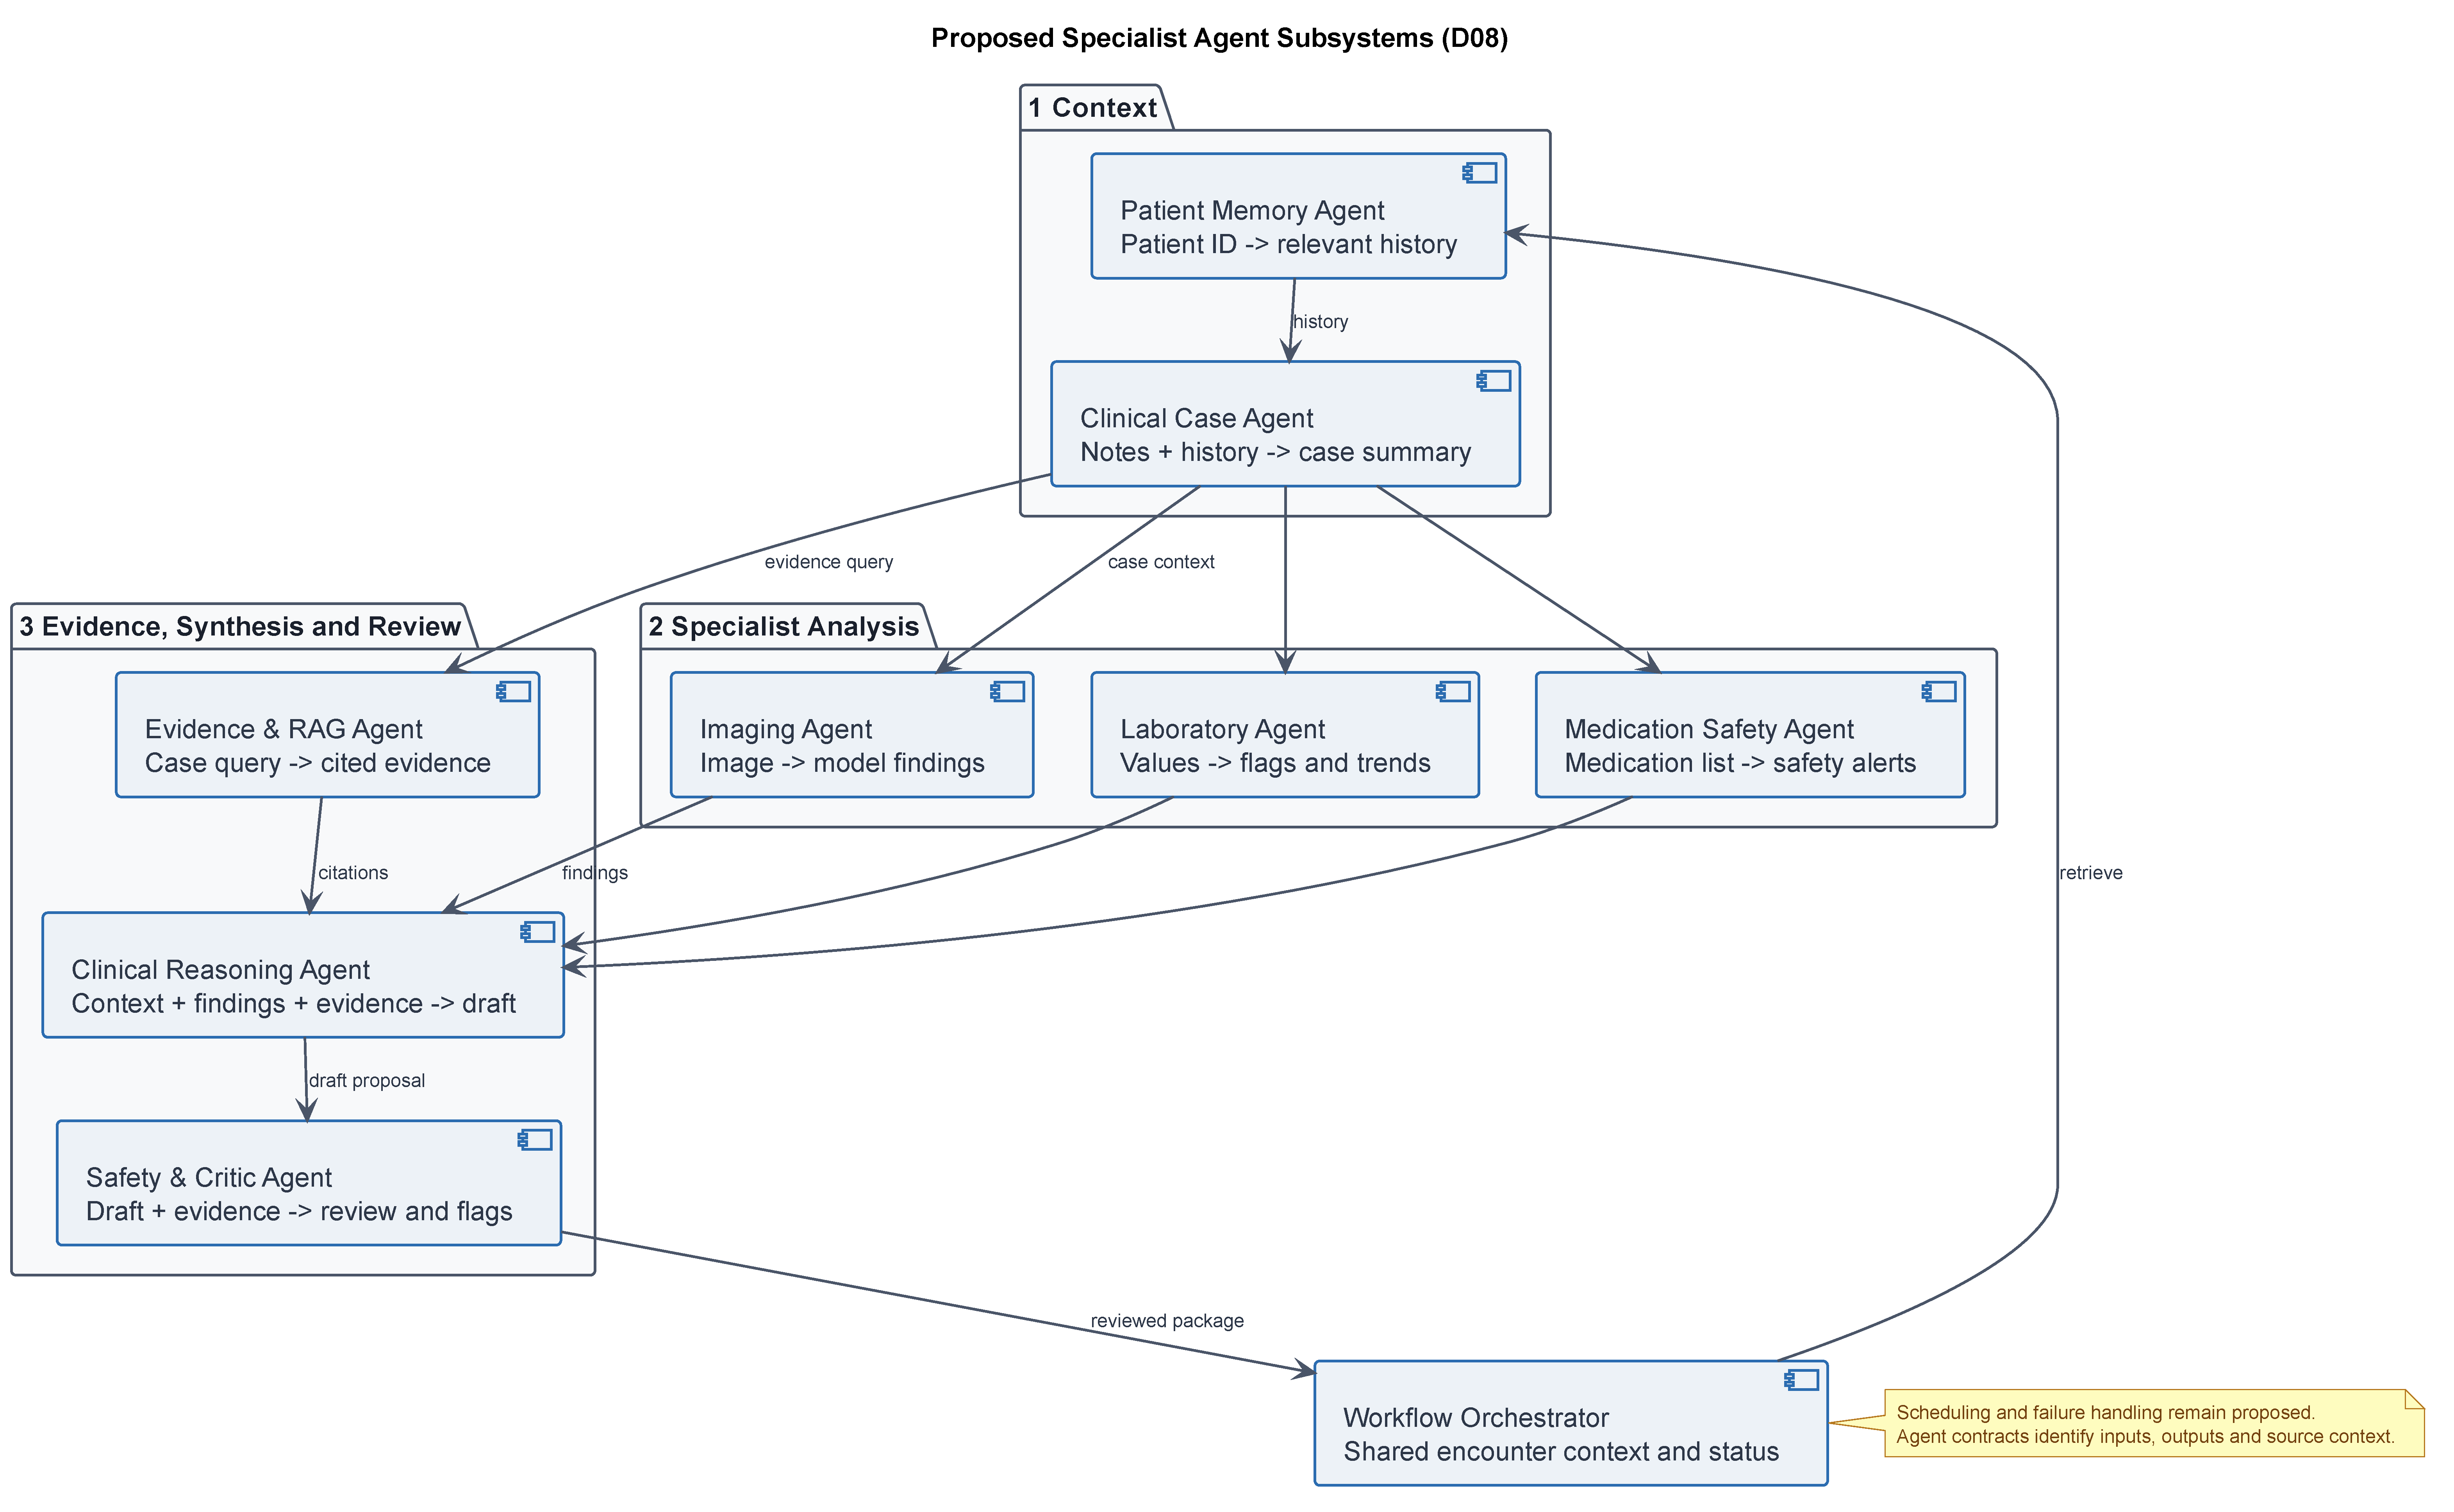
\includegraphics[width=\textwidth,height=0.80\textheight,keepaspectratio]{Figures/esha_D08_agent_subsystems.pdf}
\caption{Eight specialist agents and their case-processing handoffs.}
\label{fig:esha:d08}
\end{figure}

\begin{reporttable}
\centering
\small
\caption{Proposed specialist agent input, output, persistence and recipient contracts .}
\label{tab:esha:contracts}
\begin{tabular}{|p{0.18\textwidth}|p{0.22\textwidth}|p{0.245\textwidth}|p{0.245\textwidth}|}
\hline
Agent Name & Primary Inputs & Primary Outputs & Storage \& Recipient \\ \hline
Patient Memory Agent & \texttt{patient\_id}, encounter context & Relational history, top-$k$ semantic memories & PostgreSQL/pgvector; Orchestrator \\ \hline
Clinical Case Agent & Notes, multimodal data, retrieved history & Consolidated case representation & Working memory cache; Specialist agents \\ \hline
Imaging Agent & Radiological image tensor / file reference & Predicted pathology classes, confidence scores & Working cache; Reasoning Agent \\ \hline
Laboratory Agent & Laboratory panel values, reference ranges & Abnormal biomarker flags, trajectory trends & Working cache; Reasoning Agent \\ \hline
Medication Safety Agent & Active prescriptions, candidate drugs & Drug-drug interactions, contraindication alerts & Knowledge base; Reasoning Agent \\ \hline
Evidence \& RAG Agent & Diagnostic keywords, clinical hypotheses & Cited guideline passages, source identifiers & pgvector vector index; Reasoning Agent \\ \hline
Clinical Reasoning Agent & Consolidated case, specialist findings, evidence & Differential diagnosis draft, treatment plan & Gemini API; Safety \& Critic Agent \\ \hline
Safety \& Critic Agent & Generated draft, case context, cited evidence & Consistency evaluation, risk alerts, critique & Working cache; Presentation tier \\ \hline
\end{tabular}
\end{reporttable}

\begin{figure}[!htbp]
\centering
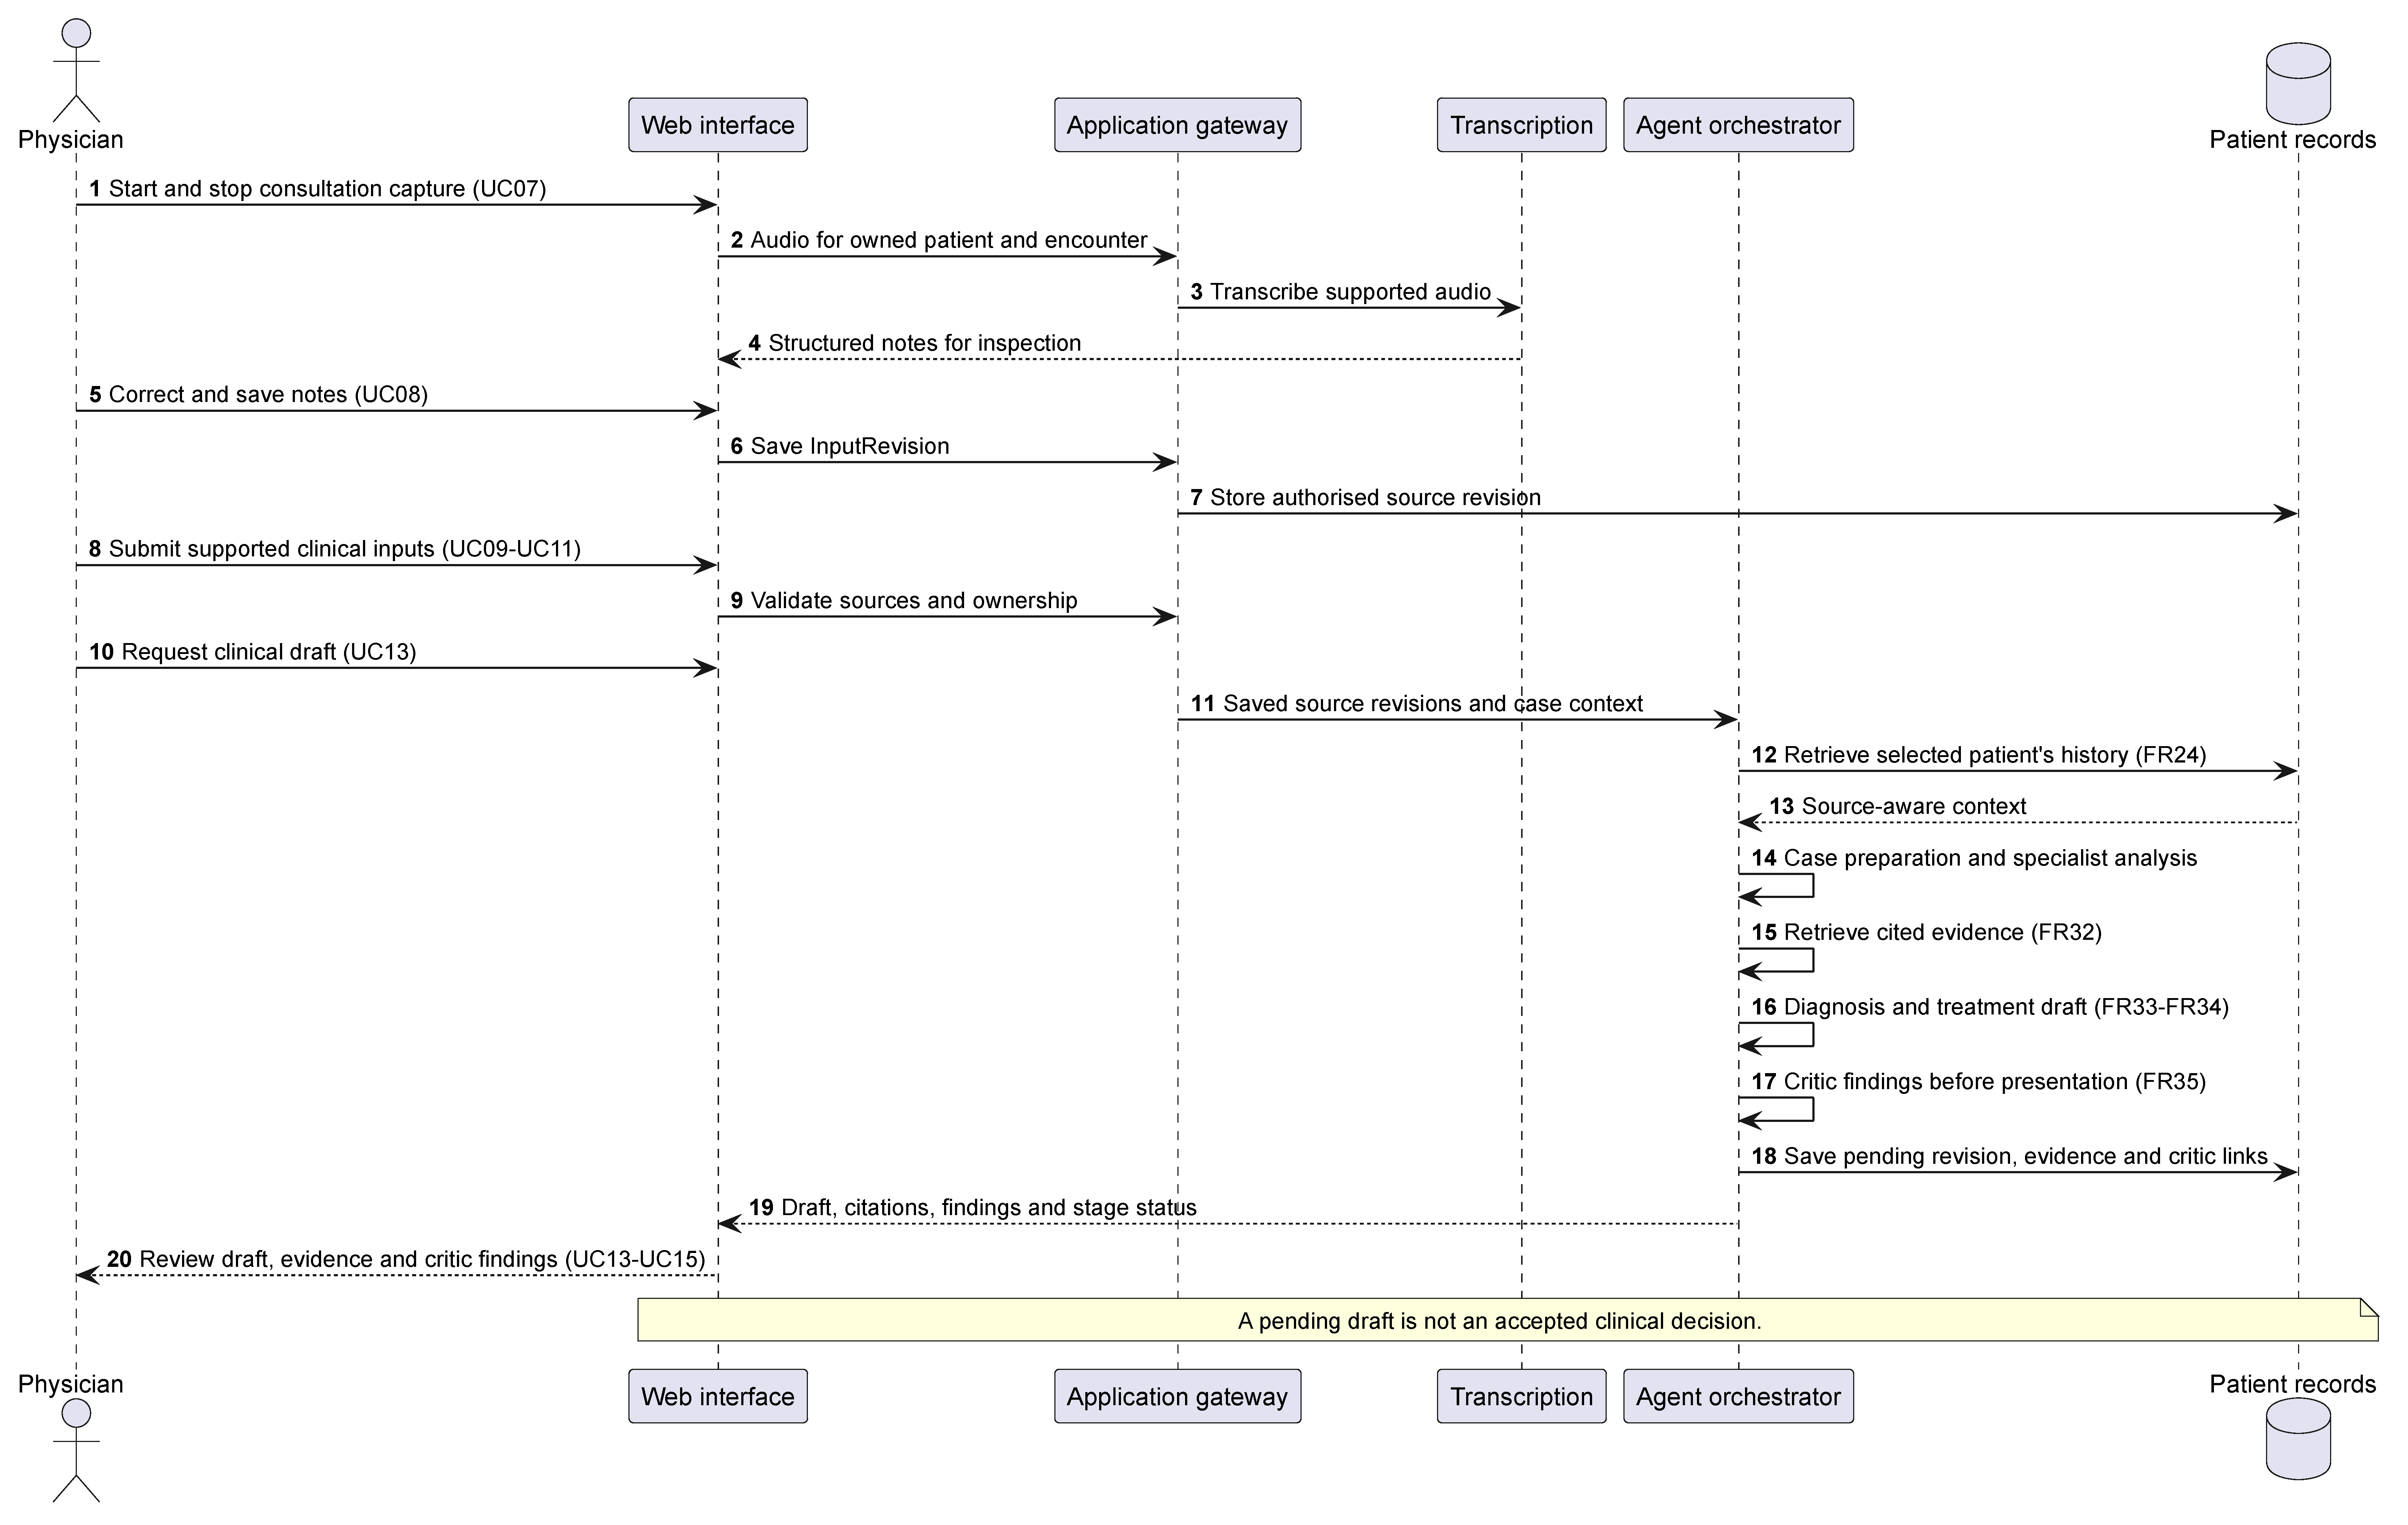
\includegraphics[width=\textwidth,height=0.80\textheight,keepaspectratio]{Figures/esha_D10_consultation_sequence.pdf}
\caption{Consultation capture, source-aware analysis and draft presentation sequence.}
\label{fig:esha:d10}
\end{figure}

\begin{figure}[!htbp]
\centering
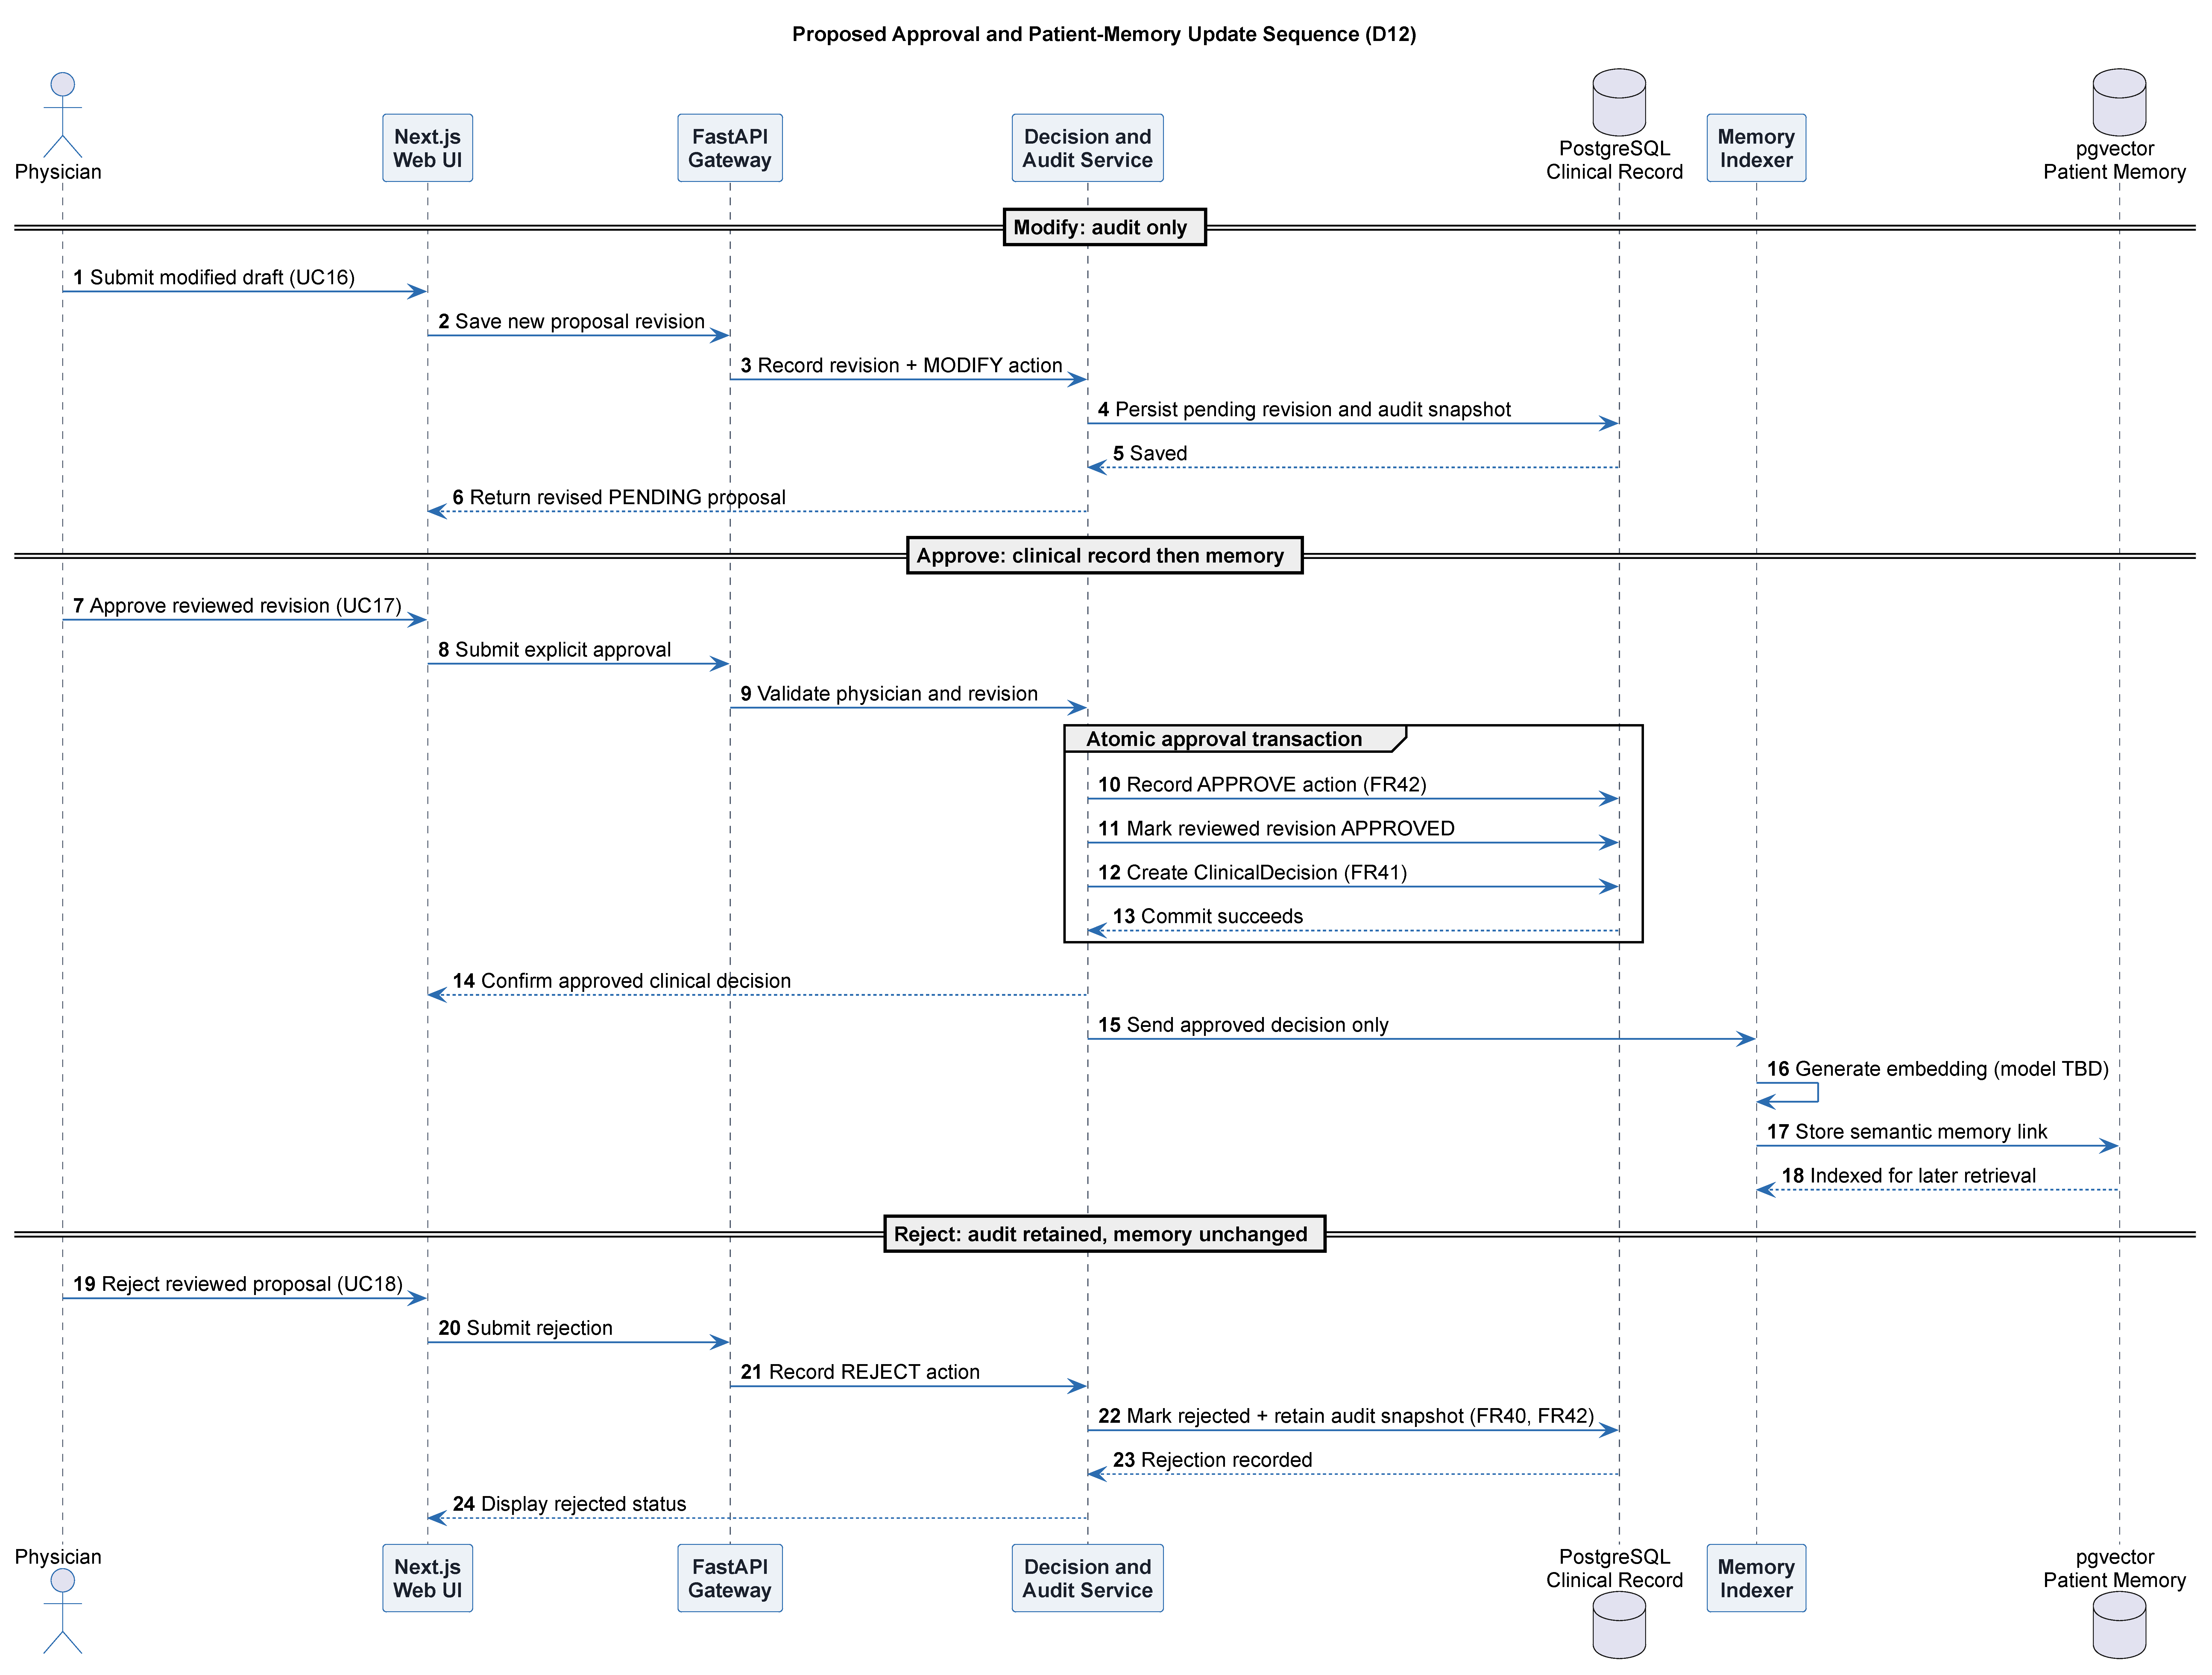
\includegraphics[width=0.96\textwidth,height=0.78\textheight,keepaspectratio]{Figures/esha_D12_memory_update_sequence.pdf}
\caption{Revision-specific physician actions, decision recording and memory indexing.}
\label{fig:esha:d12}
\end{figure}


\section{Architectural Strategies}

The architectural strategies address patient continuity, processing dependencies and accountable review rather than assuming diagnostic improvement from added components. Hybrid persistence combines explicit account, patient and encounter relationships with semantic retrieval over identifiable sources. Orchestration keeps agent responsibilities separate and coordinates their inputs before drafting. Model adapters isolate service-specific formats and errors, while transactional application services govern approval and audit recording. Table~\ref{tab:esha:decisions} records the supported technology choices, trade-offs and configuration decisions that remain open. These strategies support controlled evaluation: a simpler variant can withhold a component while retaining the same case definition and reference process. Independent processing may use asynchronous execution, but dependencies must be respected and failed analyses must remain visible. No strategy establishes guaranteed throughput, clinical safety or regulatory compliance. Its value must be assessed through implementation checks and comparative runs. The design connects engineering choices to testable behaviour while preserving the physician's responsibility for every accepted revision.

\subsection{Hybrid Relational and Vector Memory Persistence}

PostgreSQL preserves physician ownership, patient and encounter associations, input revisions, draft revisions, evidence links, review actions and accepted decisions. Foreign keys and transaction boundaries support checks that related records belong to the same case and reviewed revision. Semantic memory uses pgvector representations linked to an authorised input revision or an approved decision. This distinction permits retrieval of source observations while preventing a pending or rejected draft from being treated as an accepted clinical conclusion. Retrieval returns the originating record and its context so similarity alone does not establish clinical relevance. Historical information must remain within the selected patient's ownership boundary, and observations must remain distinguishable from earlier encounters. Embedding model, dimension and indexing configuration require selection before storage and search can be evaluated. The hybrid design retains explicit relationships alongside semantic search, but its relevance and latency must be measured rather than inferred from the presence of a vector index.

\subsection{Asynchronous Agent Orchestration and Model Runtime Segregation}

The application separates case operations from analytical work that may depend on local inference or remote services. Consultation capture, saved note revisions and physician review should retain understandable states while an analysis is pending. The orchestrator starts independent specialist tasks only after the required case context is available, then combines returned findings and failure information before drafting. Dependencies determine whether a task can run concurrently; evidence retrieval must receive the information needed to form a query. Service adapters validate payloads and distinguish timeouts, rejected inputs and unavailable resources from completed results. A partial case can remain available for inspection, but missing analysis must not be silently represented as normal findings. LangGraph and Google ADK provide candidate orchestration mechanisms, with their final division during implementation. Asynchronous execution supports this separation without establishing a measured speed improvement. Stage status should remain visible while other services finish, fail or await required case information.

\begin{reporttable}
\centering
\small
\caption{Architectural design decisions, supported choices, trade-offs and unresolved options .}
\label{tab:esha:decisions}
\begin{tabular}{|p{0.20\textwidth}|p{0.22\textwidth}|p{0.245\textwidth}|p{0.225\textwidth}|}
\hline
Design Dimension & Proposed Choice & Architectural Trade-off & Unresolved Status \\ \hline
Backend Framework & FastAPI (Python) & High-speed async I/O and native Python ML ecosystem versus separate microservices & Production server concurrency tuning TBD \\ \hline
Frontend Framework & Next.js / TypeScript & Rich React component ecosystem and streaming support versus heavier bundle size & View layout refactoring planned \\ \hline
Multi-Agent Orchestrator & LangGraph / Google ADK StateGraph & Cyclic state-graph flexibility versus increased execution graph complexity & Formal division of roles between frameworks TBD \\ \hline
Primary Reasoning Model & Google Gemini API & Advanced multimodal context window versus reliance on cloud API latency & Production model version and quotas TBD \\ \hline
Radiology Classifier & PyTorch Pre-trained Model & Validated local inference speed versus fixed diagnostic pathology label sets & Exact pre-trained model checkpoint TBD \\ \hline
Memory Storage & PostgreSQL with pgvector extension & Unified relational ACID guarantees and vector search versus dedicated vector database & Vector dimension and HNSW index tuning TBD \\ \hline
\end{tabular}
\end{reporttable}


\section{Domain Model/Class Diagram}

Figure~\ref{fig:esha:d09} presents the clinical domain classes and their associations; the complete persistence attributes are defined in Chapter~4. Physician, Patient and Encounter maintain account access, ownership and patient encounter context. ClinicalInput and InputRevision distinguish an input from its saved versions, while SpecialistFinding identifies the revision analysed. Proposal and ProposalRevision separate a draft's identity from reviewed content; ProposalInput, EvidenceItem, ProposalEvidence and CriticReview preserve its sources and assessment. PhysicianAction records the actor, revision and physician review event, and ClinicalDecision stores the explicitly accepted content. SemanticMemory links authorised source revisions or approved decisions to their representations. EvaluationCase, EvaluationRun and EvaluationOutput keep research case inputs, configurations and outputs identifiable. Application services coordinate retrieval, analysis and transactional approval rather than assigning unrestricted database writes to agents. The model aligns with the eighteen-entity dictionary while distinguishing service behaviour from stored records. Class associations specify domain entity relationships; their integrity must be verified when persistence is implemented.

\begin{figure}[!htbp]
\centering
\includegraphics[width=\textwidth,height=0.80\textheight,keepaspectratio]{Figures/esha_D09_domain_classes.pdf}
\caption{Domain classes with ownership, revision, evidence and decision associations.}
\label{fig:esha:d09}
\end{figure}


\section{Policies and Tactics}

Local policies govern account access, source handling and state transitions within the architecture. The physician's authenticated identity is checked against the selected patient before any related record is read or processed. Saved revisions preserve the clinical content used for analysis and review, while source links identify the findings and passages supporting each draft. Review actions retain their actor, time and revision; approval records matching accepted content in a transaction, and modification or rejection does not create a decision. Evidence and critic findings remain inspectable even when they identify insufficient support. Analytical errors must be returned with their stage and source context so an incomplete operation cannot appear successful. Semantic retrieval distinguishes authorised observations from approved conclusions and excludes unaccepted draft content from accepted-decision memory. These policies provide verification targets for implementation and research cases. Checks must cover incorrect ownership, stale revisions and missing evidence as well as successful workflow operations.

\subsection{Physician Review Boundary and Audit Immutability Policy}

Figure~\ref{fig:esha:d11} distinguishes pending, modified, approved and rejected draft states. Every generated draft begins pending physician review. Modification creates a saved revision and records a MODIFY action while leaving the draft unapproved. Approval requires the authenticated physician to own the patient and review the exact saved revision. A transaction records the APPROVE action, accepted revision and matching ClinicalDecision, preventing an action from accepting different content. Rejection records a REJECT action and retains the review history without creating an accepted decision. Audit entries preserve the actor, time, encounter and revision rather than replacing earlier review events. Pending and rejected revisions remain available as drafts and history, but cannot enter accepted-decision memory. Authorised clinical input revisions can still provide historical context through their separate source links. These controls define the decision boundary; concurrency, failed transactions and repeated requests must be checked during implementation to confirm that their recorded outcomes preserve the required relationships.

\begin{figure}[!htbp]
\centering
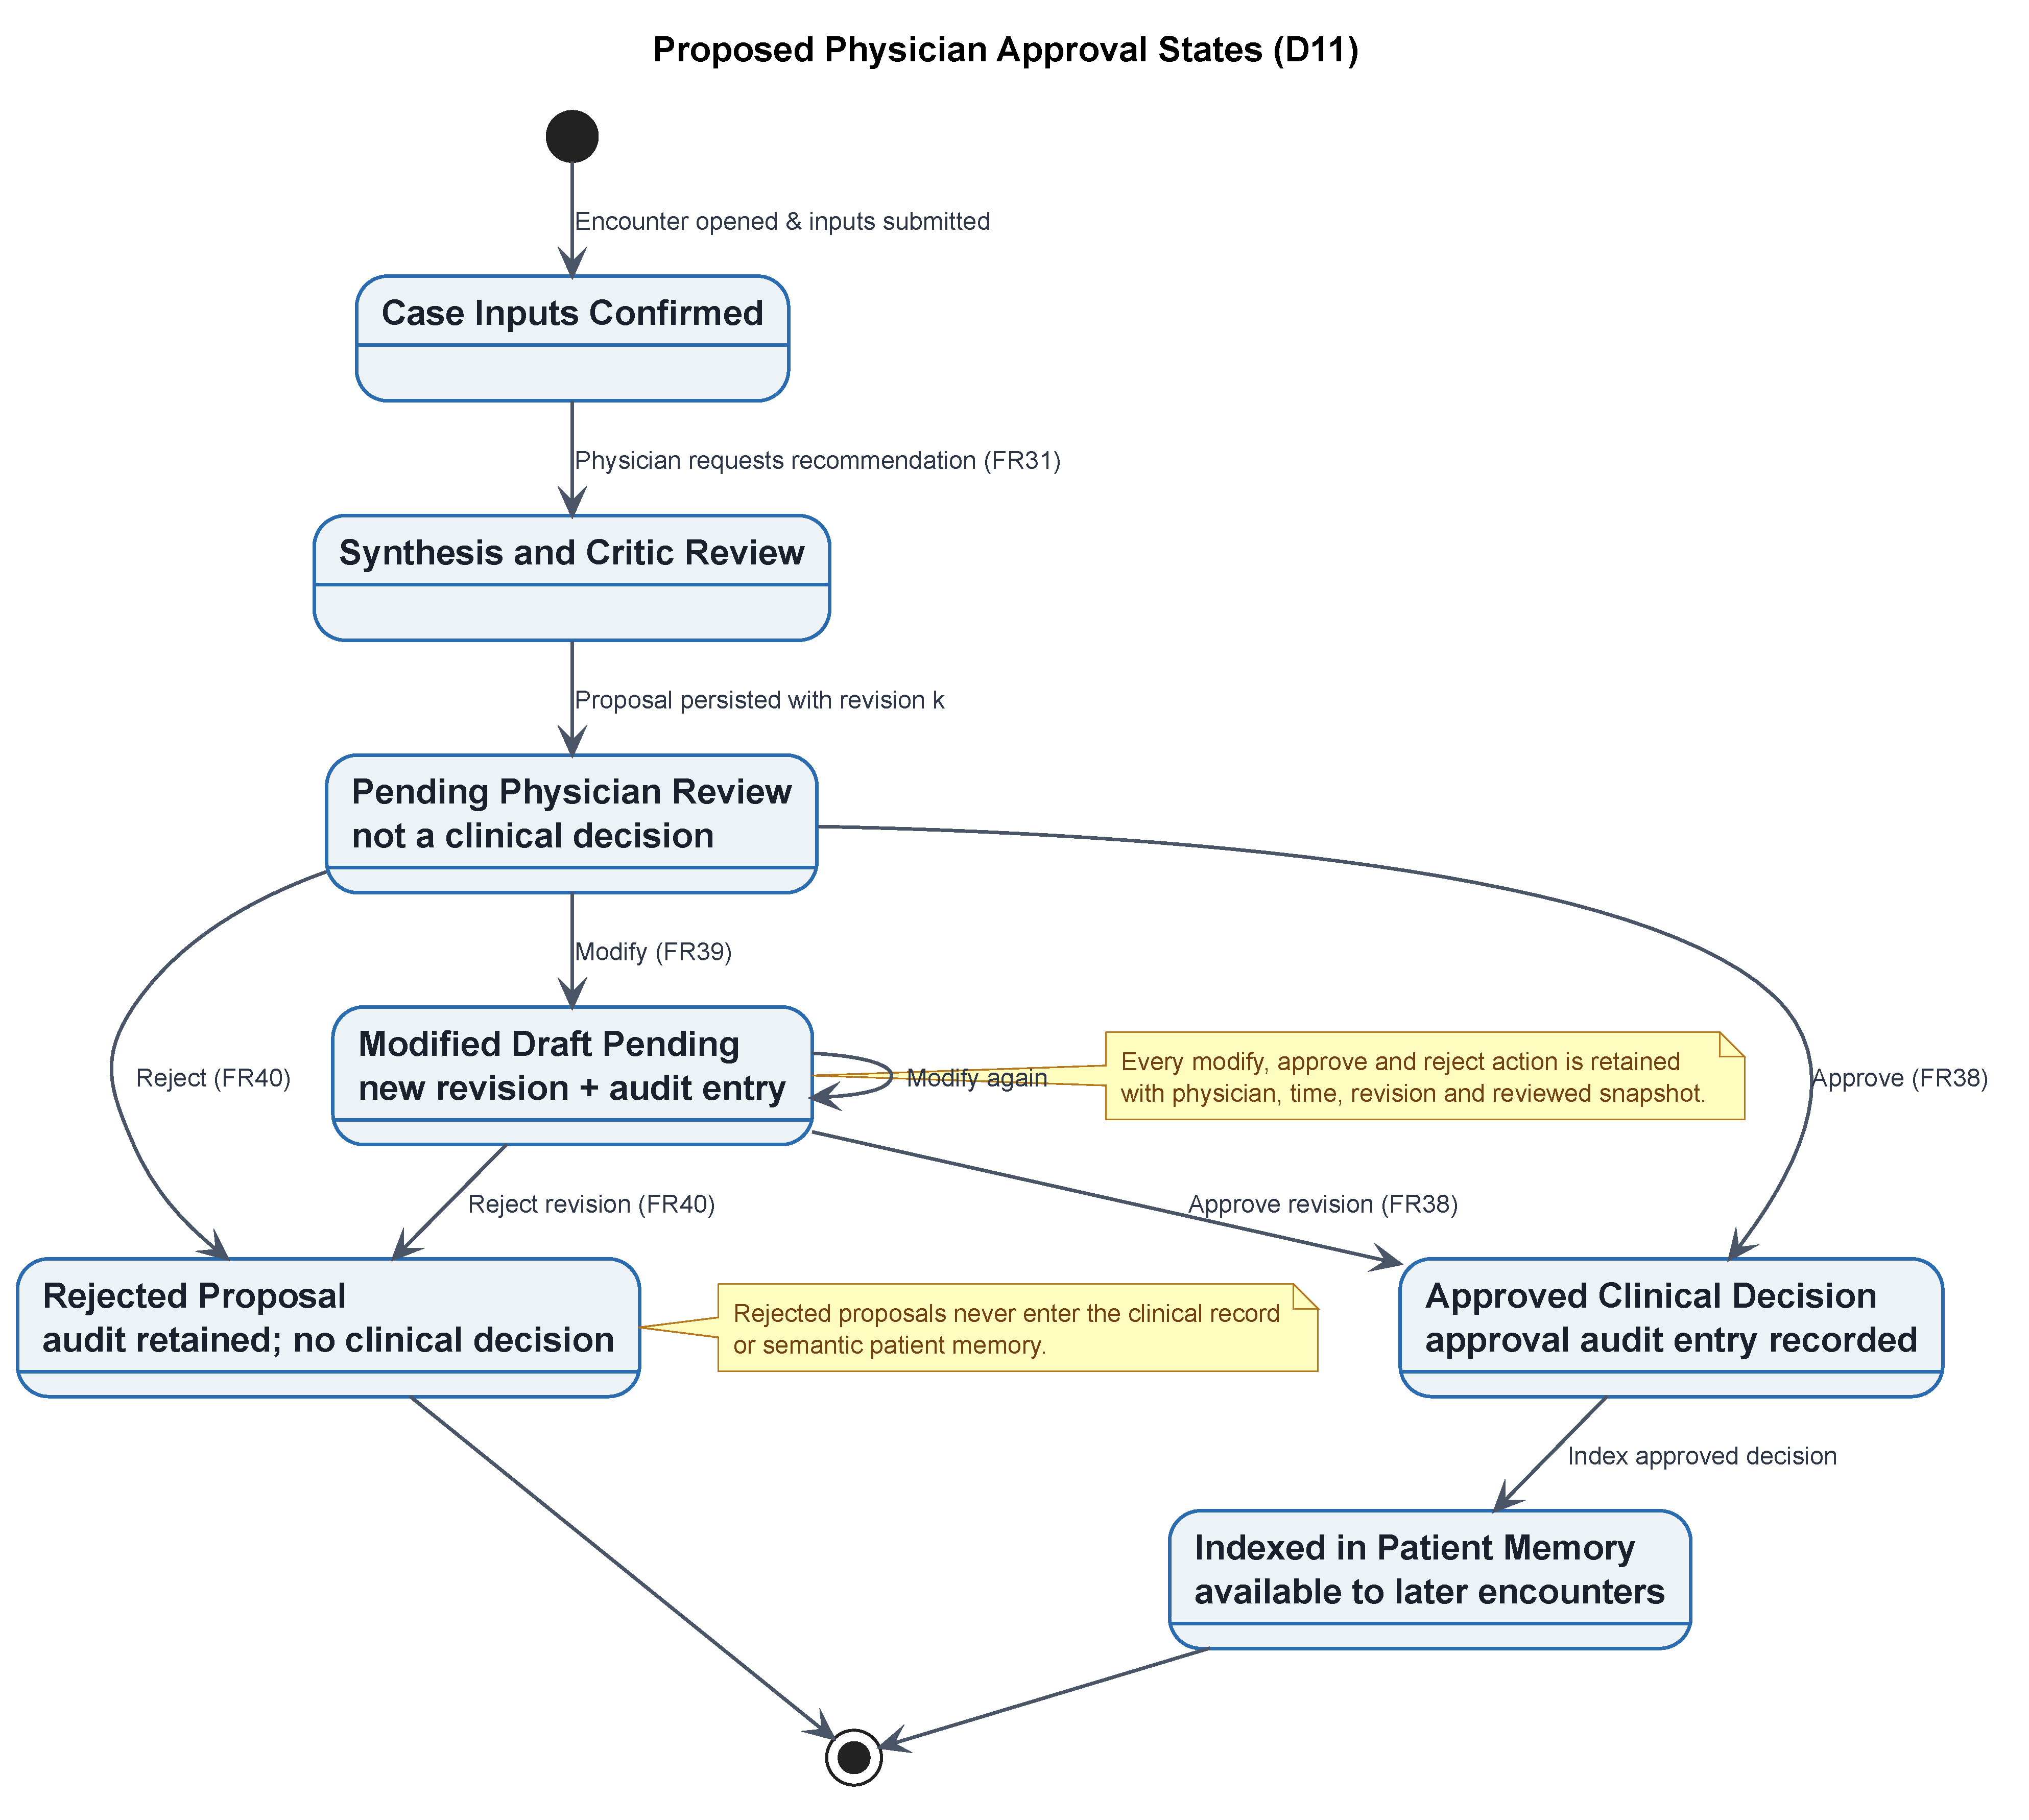
\includegraphics[width=0.88\textwidth,height=0.76\textheight,keepaspectratio]{Figures/esha_D11_approval_states.pdf}
\caption{Physician-controlled draft states and explicit approval transitions.}
\label{fig:esha:d11}
\end{figure}

\subsection{Grounded Clinical Evidence Citation and Critic Verification Tactic}

The Evidence and RAG Agent returns supporting passages with source identifiers and citations rather than only an explanation. The Clinical Reasoning Agent uses these passages alongside patient context and specialist findings when preparing a diagnosis and treatment draft. Evidence links identify the saved revision they support, allowing the physician to inspect the relationship between a recommendation and its sources. The Safety and Critic Agent examines the draft for insufficient support, inconsistency and safety concerns before presentation. Critic findings retain their assessed revision and appear alongside the draft, including concerns that remain unresolved. Missing evidence must be shown as missing rather than replaced with fabricated citations, and critic review must not be described as proof of correctness. Physician approval remains necessary regardless of the critic outcome. These tactics complete the architecture's review pathway and establish comparison targets for evidence support and critic contribution; their effectiveness requires implemented workflows and measured evaluation.

\section{Conclusion}

The design translates Zeest's requirements into a physician interface, application gateway, coordinated agents, supporting analytical services and hybrid memory. Defined boundaries preserve patient ownership and distinguish source observations, specialist findings, generated drafts and accepted decisions. Revision relationships connect the information used for analysis with the evidence and critic findings presented during review. Application services govern approval and audit recording, while analytical agents remain responsible for preparation, retrieval and recommendations. The domain model and behavioural diagrams provide complementary views of these responsibilities and their permitted transitions. Component adapters and visible failure states support integration without implying that every candidate resource is already available. The architecture also accommodates controlled research comparisons by retaining case definitions, configurations and outputs independently of clinical decision records. Implementation must validate these contracts, transaction boundaries and failure paths before performance or clinical-value claims can be made. The resulting design provides a coherent development foundation while preserving physician authority and the limits of the current research scope.

\endgroup
